\title{SDN Project Proposal}
\author{
        David Poliakoff \\
        David Ozog \\
}
\date{\today}

\documentclass[12pt]{article}
\usepackage{graphicx}
\usepackage{amsmath}
\newcommand{\HRule}{\rule{\linewidth}{0.3mm}}

\begin{document}
\maketitle
\centerline{\HRule}

%\begin{abstract}
%This is the paper's abstract \ldots
%\end{abstract}

\section*{Problem:}
\label{problem}
A great deal of flexibility is available within the SDN paradigm 
where there is a complete separation of the networking data plane from the control plane via
software abstractions.  One area that is left to be explored is how large-scale computational applications
can benefit from the control abstraction layers that SDN provides.
We believe that having the ability to reconfigure the network 
at application runtime can provide opportunity for optimizations that were 
previously not possible.  Furthermore, event counters and statistics
that are provided by OpenFlow switches could provide valuable
information for computational load balancing that is not available 
without such functionalities.   

An example of where this might be applicable is in applications that utilize
a Partitioned Global Address Space (PGAS), in which data is spread
across a distributed memory cluster in such a way that is abstracted from
the programmer.   For instance, the Global Arrays (GA) library provides a friendly
API for doing ``shared-memory style" programming on distributed memory commodity clusters.  
Specifically, one can easily do multi-dimensional matrix operations with a single call across
a collection of distributed machines.

Unfortunately, this complicates the issue of exploiting and optimizing data affinity
in many applications.  For example, the coupled cluster module of NWChem 
(built on PGAS/GA) performs large tensor contractions by splitting the global 
data space into smaller \textit{tiles}.  These tiles are gathered from ``relatively unknown" locations
in the PGAS and operated on locally with multiple iterations.  Unfortunately, it can be difficult for the application
to adapt to situations where data locality is poor.  With the power to measure 
network counters and reconfigure the network on the fly, problems such as this can 
potentially be alleviated.


\section*{Solution:}
\label{solution}
\begin{figure}[t]
\centerline{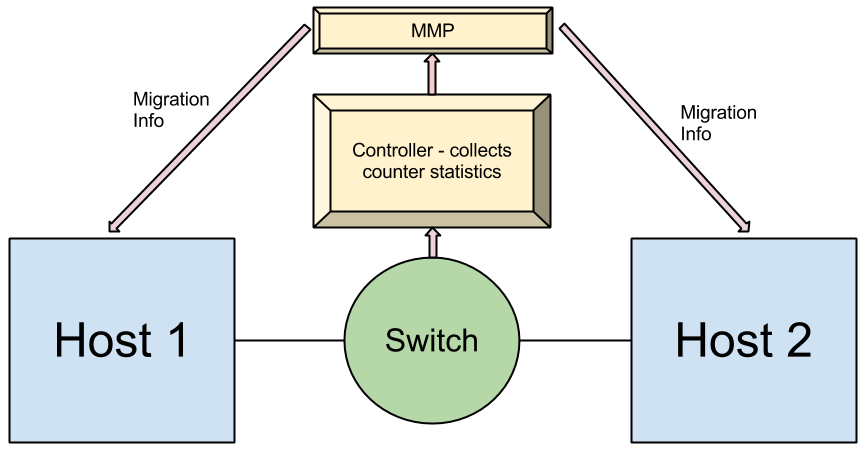
\includegraphics[width=4.0in]{img/toy_arch.png}}
\caption{The simple topology and software architecture diagram of our first toy application.  The Controller 
will gather flow statistics (in units of bytes per flow per second) at a frequency $f$. Relevant data is then
shipped to the Migration Management Process (MMP) which makes decisions about host data migration, and sends the
decisions to the hosts.}
\label{fig:toy_arch}
\end{figure}
We propose to develop a simple synthetic application which performs a global operation on data
that is intentionally unoptimized for locality.  Because this problem can be difficult for application
programmers to solve based only on application-level information, we will design and develop a simple
%example application where SDN counters and re-configurations are used to improve data locality on the 
example application where SDN provided network traffic statistics will be used to reconfigure data to improve locality on the
fly.  The application will directly communicate with the controller process (or a proxy on its behalf)
to inform the application where data should be migrated in order to improve data locality for subsequent
operations and/or iterations (see Figure~\ref{fig:toy_arch}).

\subsubsection*{Application:}
\label{application}
The synthetic application we will develop for this project will do computation on multiple sets of data.
The application will require the entirety of the set of data in order to do some computation.  In the 
beginning it will get the entire set by doing remote data access.  As the application progresses,
it will replace the remote data accesses with migrations of data in response to a reorganization algorithm
run on a remote process, which we will call the (Migration Management Process) MMP.  Both the MMP and the 
application will be written in Python for simplicity.

We will develop this application in a series of steps, beginning with the simplest toy problem possible, 
as shown in Figure~\ref{fig:toy_arch}.
In this version, we will use a single switch and two hosts with only two sets of data, $A$ and $B$, evenly
distributed between the hosts.  After gathering switch statistics and making the necessary migrations, then
the system succeeds if all of the $A$ dataset is located on host 1 and all of the $B$ dataset is on host 2
(as in Figure~\ref{fig:toy2}).

It is clear that certain application parameters (such as computation/communication ratios, data migration size,
etc) will play a direct role in the behavior of the system.  The parameters need to be specified, evaluated, and
possibly tuned.  For now, we will keep a running list of parameters that we will control and monitor:
\begin{enumerate}
  \item Computation time and/or FLOPS per iteration (in the application)
  \item Size of data (in bytes) which is operated on and migrated (initially, we keep data unit size uniform)
  \item Computation/Delay between iterations (initially, zero)
\end{enumerate}

\begin{figure}[t]
\centerline{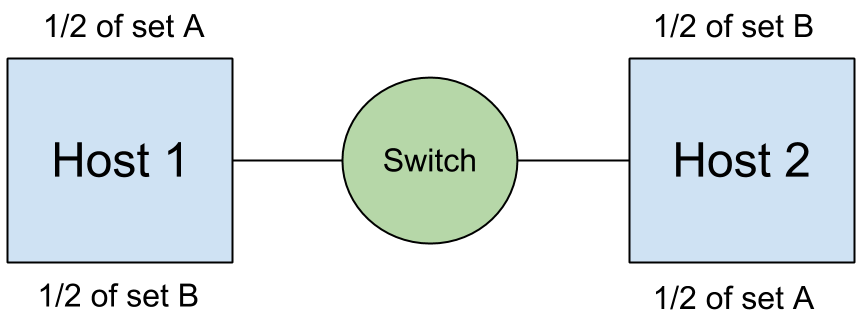
\includegraphics[width=3.0in]{img/toy1.png}}
\caption{Simple topology for out toy application with an initial data distribution}
\label{fig:toy1}
\end{figure}

\begin{figure}[t]
\centerline{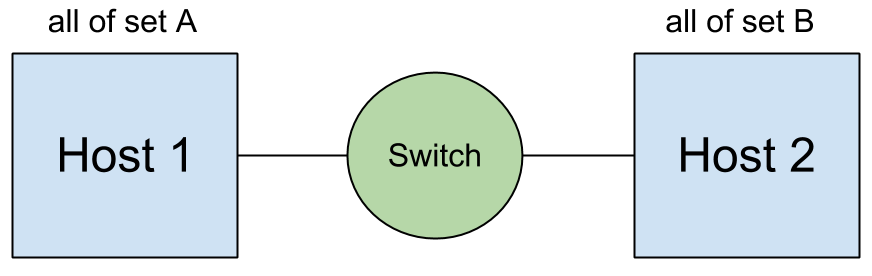
\includegraphics[width=3.0in]{img/toy2.png}}
\caption{The desired final data distribution for the above toy application}
\label{fig:toy2}
\end{figure}


\subsubsection*{Controller:}
\label{controller}
The controller will periodically query a set of switches for flow statistics. In the toy example this will be one switch.
These statistics will be shipped off to the MMP to make decisions about data migration.  The frequency with 
which statistics are collected will need to be tuned.  In our toy example, the simplicity of data layout should
lead to a regular traffic pattern until migration occurs.  This is because we will initially require the 1st host
to remotely get $B$ data, and the second host to remotely get $A$ data in an iterative loop, without doing migration.
Repeatedly performing the same operations should produce a regular traffic pattern. Starting with a low sampling frequency, 
we will increase the frequency until the observed traffic pattern stabilizes at which point we will have an appropriate 
sampling rate.%chicken


\subsubsection*{MMP:}
\label{mmp}
The role of the MMP is to take as input relevant data from the OpenFlow table statistics counters,
and output data migration decisions based on the goal of reducing network traffic by increasing data 
locality.  We will keep this decision making algorithm as simple as possible: if the flow rate 
(in bytes per second) is above a threshold (which initially we will have to determine empirically and 
tune), then we will migrate data.  This algorithm we will refer to as the \textit{reaction function}.  

One complication that arises in this context is how we will 
associate a particular dataset (for example, $A$ in Figure~\ref{fig:toy1}) with a measured flow.  We have
decided to require each unique dataset to send/receive on a particular port.  That way, we know which
dataset corresponds to a flow counter by simply knowing the port.  If this does not work out, there may
be other approaches such as including this information in the packet headers.

\begin{figure}[t]
\centerline{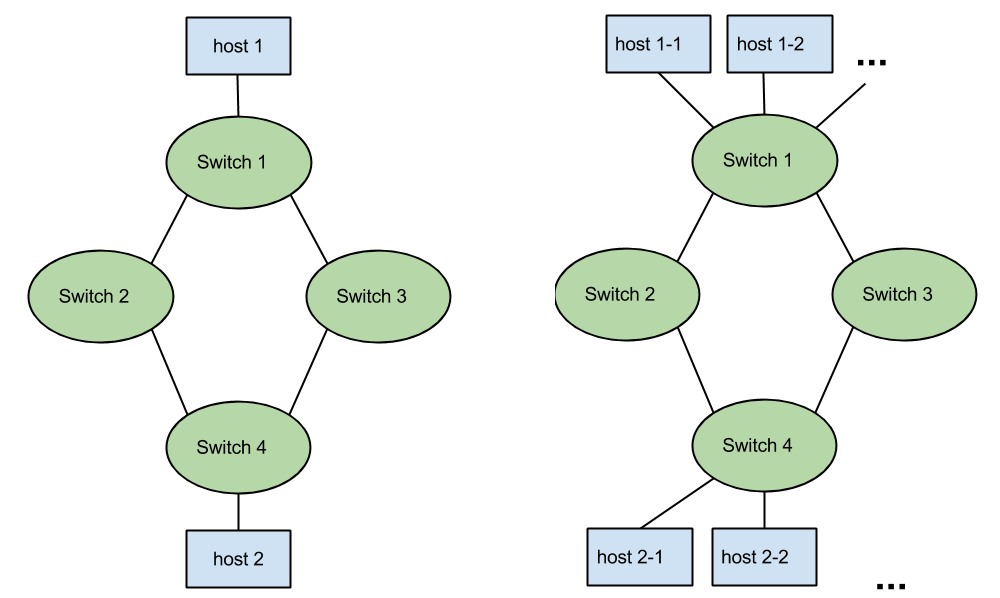
\includegraphics[width=4.0in]{img/topo_comp.png}}
\caption{If all goes well, we will consider a slightly more complicated topology for a toy synthetic application (left) and then the  same application with multiple hosts (right). In these cases we will first limit our measurement points
to Switch 3.  If that goes well, we will consider an approach which intelligently chooses
measurement points in more complicated networks based on a modified max-flow min s-t cut algorithm.}
\label{fig:topo_comp}
\end{figure}


\section*{Plan:}
\label{plan}
\begin{figure}[t]
\centerline{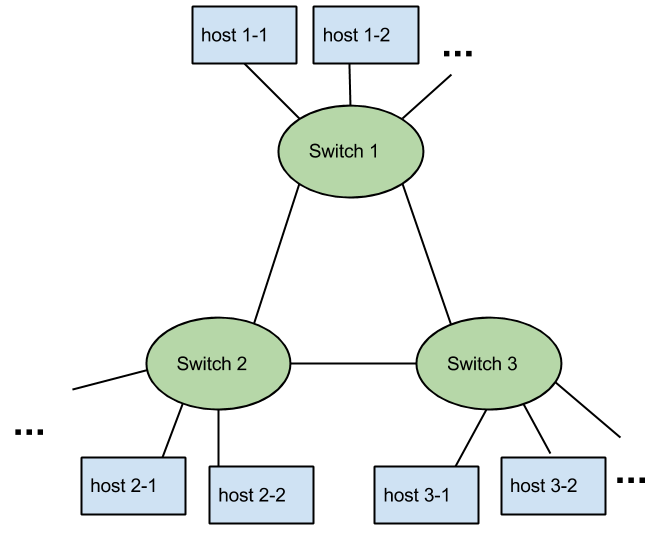
\includegraphics[width=3.0in]{img/topo.png}}
\caption{Final goal: a simple topology for synthetic application on the testbed}
\label{fig:topo}
\end{figure}
First, we will implement and evaluate our solution for the simple toy problem shown in 
Figure~\ref{fig:toy1}.  Second, we will explore a slightly more advanced network topology 
as shown in Figure~\ref{fig:topo_comp}.  We will begin by constructing a small \texttt{mininet} configuration that mimics the UO testbed
that will soon be available (Figure~\ref{fig:topo}).  Then, we will work to correlate
inter-host traffic with application activity in the context of an application working in 
a global memory space.  If the multi-switch topology proves to be too difficult, we can 
start with a single switch and build upon that.  By constraining our simulated network to the
triangle switch, we hope to transition to the testbed environment as gracefully as possible.  However,
it will suffice to run our experiments within a \texttt{mininet} network only if need be.

Specifics of the more advanced approach still need to be worked out.  For instance, we are not sure if host-to-host
traffic statistics will be available in the OpenFlow switch flow tables (though we are pretty sure they
are...).  So it is yet to be determined whether our traffic matrix algorithm will be on host-to-host
traffic:

$
M = \bordermatrix{~ & h_1 & h_2 & h_3 & h_4 ... \cr
                  h_1 & 0 & a & b & c\cr
                  h_2 & a' & 0 & d & e\cr
                  h_3 & b' & d' & 0 & f\cr
                  h_4 & c' & e' & f' & 0\cr}
\vspace{5mm}
$
\\
\vspace{3mm}
\noindent or switch-to-switch traffic:

$
M = \bordermatrix{~ & s_1 & s_2 & s_3 \cr
                  s_1 & 0  & a & b \cr
                  s_2 & a' & 0 & c \cr
                  s_3 & b' & c' & 0 \cr}
$
\\
\vspace{3mm}

There is also the question of whether to work with per-flow counters, per-port counters, or both.

As a side note, we will be using a publicly viewable Git repository for holding version controlled code.

\vspace{10mm}

\section*{Timeline:}
\label{timeline}
\begin{center}
  \begin{tabular}{ l || c }
    \hline
    Date & Milestone \\ \hline \hline
    Week 4  & Simple mininet topology w/ counters per flow and per port \\ \hline
    Week 5  & Synthetic application in place with measurably poor data locality \\ \hline
    Week 6  & Structures for counters of relevant traffic data (traffic matrix) \\ \hline
    Week 7  & Analysis/algorithm for traffic data/migration decisions in place \\ \hline
    Week 8  & Data migration based on traffic analysis \\ \hline
    Week 9  & Performance comparison and evaluation \\ \hline
    Week 10 & Presentation, demonstration, discussion \\ 
    \hline
  \end{tabular}
\end{center}


\section*{Deliverables:}
\label{deriverables}
\begin{enumerate}
\item A synthetic application that performs a global operation (reduction) on data with poor locality
\item A controller / analyzer that collects relevant counter data and flow measurements and correlates them with application operations
\item A performance evaluation framework for this system
\item A presentation / demonstration of the project
\end{enumerate}



%\bibliographystyle{abbrv}
%\bibliography{SDN_Project_proposal}

\end{document}
This is never printed
